\documentclass[12pt]{article}
\usepackage[spanish, english, es-tabla]{babel}
\usepackage[utf8]{inputenc}
\usepackage[left = 2cm, right = 2cm, bottom = 2cm, top = 3cm]{geometry}
\usepackage{amsmath, amssymb}
\usepackage{graphicx}
\usepackage{hyperref}
\usepackage{listings}
\usepackage{courier}

\usepackage[dvipsnames]{xcolor}

\renewcommand{\lstlistingname}{Código}
\renewcommand{\lstlistlistingname}{Listado de códigos}

% https://tex.stackexchange.com/questions/60209/how-to-add-an-extra-level-of-sections-with-headings-below-subsubsection
\newcommand{\subsubsubsection}[1]{\paragraph{#1}\mbox{}\\}
\setcounter{secnumdepth}{4}
\setcounter{tocdepth}{4}

% Configure lstlisting
\definecolor{codegreen}{rgb}{0,0.6,0}
\definecolor{codegray}{rgb}{0.5,0.5,0.5}
\definecolor{codepurple}{rgb}{0.58,0,0.82}
\definecolor{backcolour}{rgb}{0.95,0.95,0.92}

\lstdefinestyle{mystyle}{
	backgroundcolor=\color{backcolour},   
	commentstyle=\color{codegreen},
	keywordstyle=\color{magenta},
	numberstyle=\tiny\color{codegray},
	stringstyle=\color{codepurple},
	basicstyle=\ttfamily\footnotesize,
	breakatwhitespace=false,         
	breaklines=true,                 
	captionpos=t,                    
	keepspaces=true,                 
	numbers=left,                    
	numbersep=5pt,                  
	showspaces=false,                
	showstringspaces=false,
	showtabs=false,                  
	tabsize=2
}

\lstset{style=mystyle}


\begin{document}
	\selectlanguage{spanish}
	
	\title{Proyecto 1. Procesado de imágenes con \texttt{MATLAB} \\ \textit{\textbf{\large Máster Universitario en Ingeniería de Telecomunicación}} \\ \textit{\large Procesado de señales acústicas e imágenes}}
	\author{Enrique Fernández Sánchez \\ Link al código: \href{https://github.com/Raniita/image-processing-matlab}{Github: Raniita/image-processing-matlab}}
	
	\maketitle
	
	\tableofcontents
	
	%\addcontentsline{toc}{section}{Listado de códigos}
	\lstlistoflistings
	
	\pagebreak
	
	\section{Anonimizado}
	
	\noindent En este ejercicio tenemos que realizar técnicas de anonimizado para recortar la información a procesar de la imagen \ref{img: anonimizado src}, para ello podemos aplicar una técnica de máscara binaria o bien seleccionar manualmente la parte de la imagen a procesar.
	
	\begin{figure}[h]
		\begin{center}
			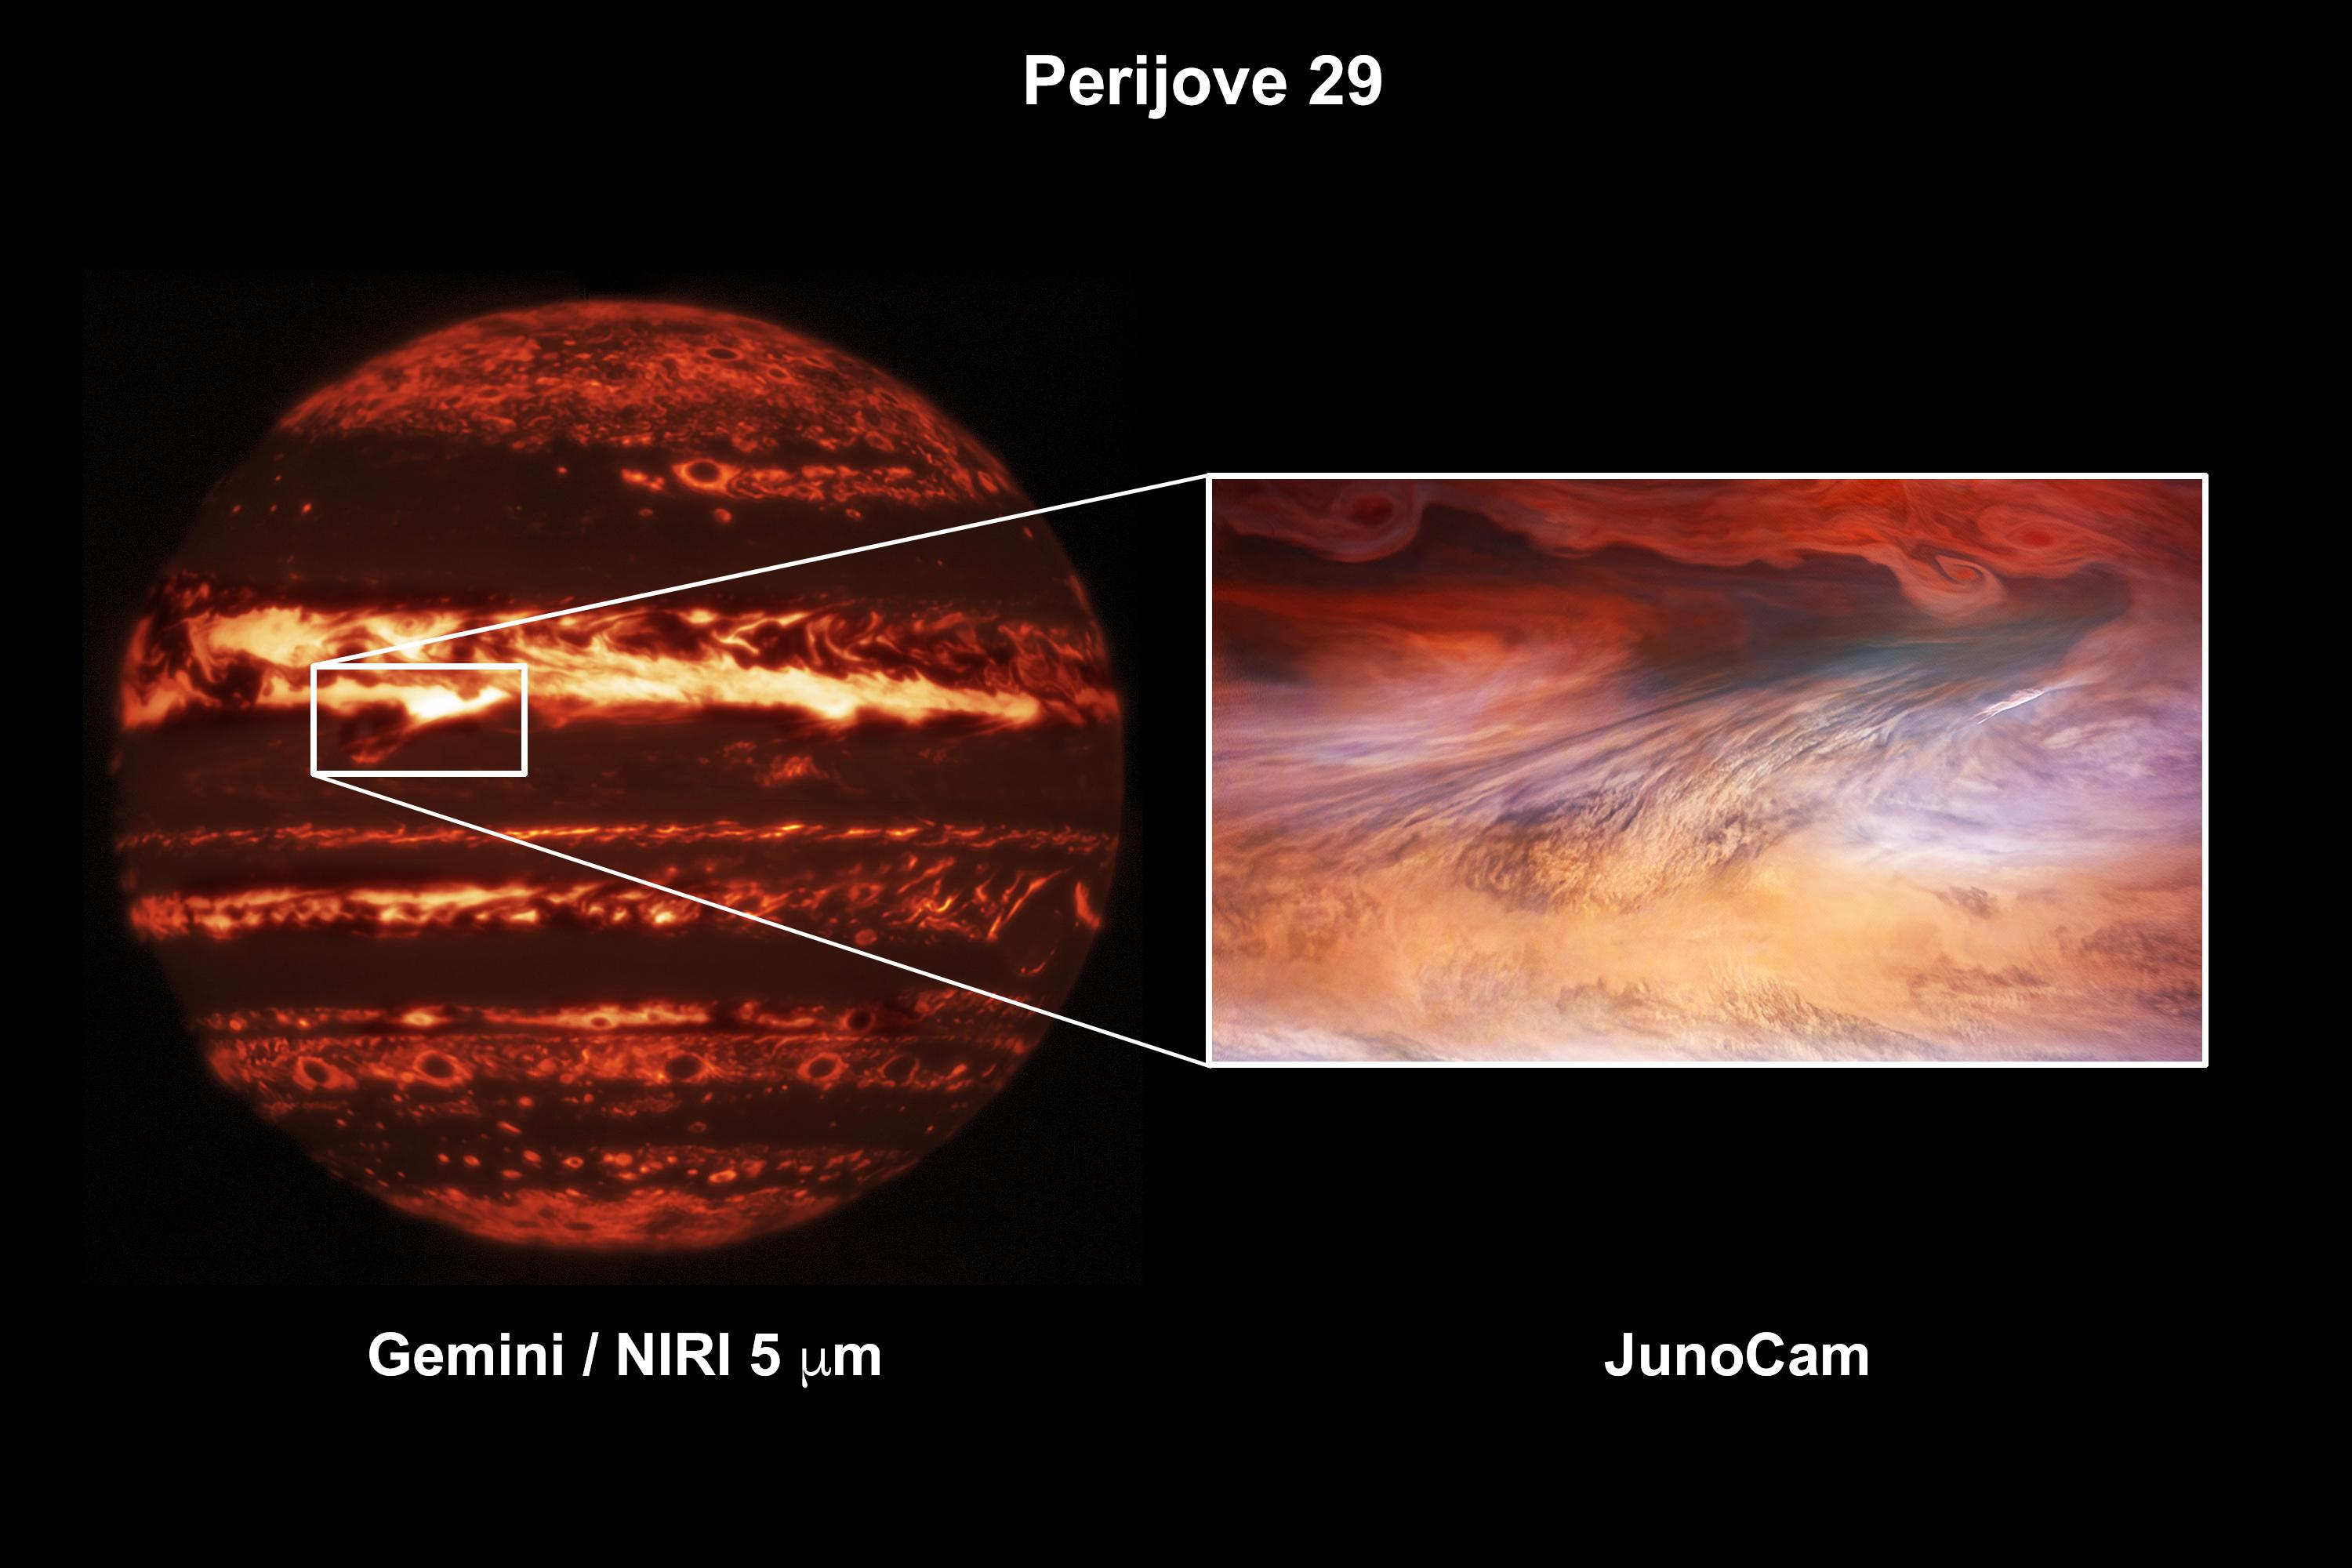
\includegraphics[width=0.9\textwidth]{img/anonimizado.jpg}
			\caption{Imagen inicial anonimizado}
			\label{img: anonimizado src}
		\end{center}
	\end{figure}

	\noindent En mi implementación, he optado por realizar una selección manual de la zona a recortar. Sin embargo, si tuviéramos que procesar muchas imágenes diferentes, la mejor opción sería realizar una máscara binaria, ya que así podríamos aplicarla de manera automática (sin intervención manual del usuario). \\
	
	\noindent El código implementado sería el siguiente:
	
	\begin{lstlisting}[language=Matlab, caption={Implementación anonimizado con MATLAB}]
% 1 - Anonimizado
% Enrique 
% Ref: https://es.mathworks.com/help/images/ref/imcrop.html
clear;

% Cargamos la imagen
img = imread('anonimizado.jpg');


% Representamos la imagen original
figure
imshow(img);
title('Imagen inicial (sin recortar)')

% Recortamos la imagen con un rectangulo
[crop_img, rect_crop] = imcrop(img);

% Manera automatica
%rect_crop = [120 300 2750 1400];    % [xmin ymin width height]
%crop_img = imcrop(img, rect_crop);

% Comparativa imagen original vs imagen recortada
figure
%suptitle('Imagen Anonimizada')

subplot(1,2,1)
imshow(img)
title('Imagen inicial')

subplot(1,2,2)
imshow(crop_img)
title('Imagen recortada utilizando un rectangulo')
	\end{lstlisting}

	\vspace{10px}

	\noindent Una vez ejecutado el código, tendremos como salida una comparativa entre la imagen inicial (ver figura \ref{img: anonimizado src}) y la imagen recortada:
	
	\begin{figure}[h]
		\begin{center}
			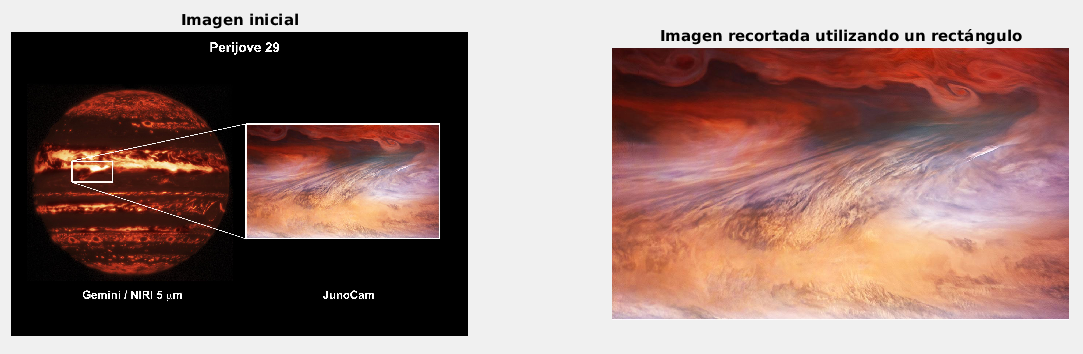
\includegraphics[width=1\textwidth]{img/anonimizado_output.png}
			\caption{Figura de salida al ejecutar script de MATLAB \texttt{anonimizado.m}}
			\label{img: anonimizado output}
		\end{center}
	\end{figure}
	
	\pagebreak
	
	\section{Contraste}
	
	\pagebreak
	
	\section{Iluminación}
	
	\pagebreak
	
	\section{Suavizado}
	
	\pagebreak
	
	\section{Realzado}
	
	\noindent En este ejercicio tenemos que aplicar técnicas de realzado para obtener más detalles en la imagen X. Para ello, aplicaremos diferentes filtros, con el objetivo de resaltar los cambios entre las diferentes zonas de color de la imagen.
	
	\begin{figure}[h]
		\begin{center}
			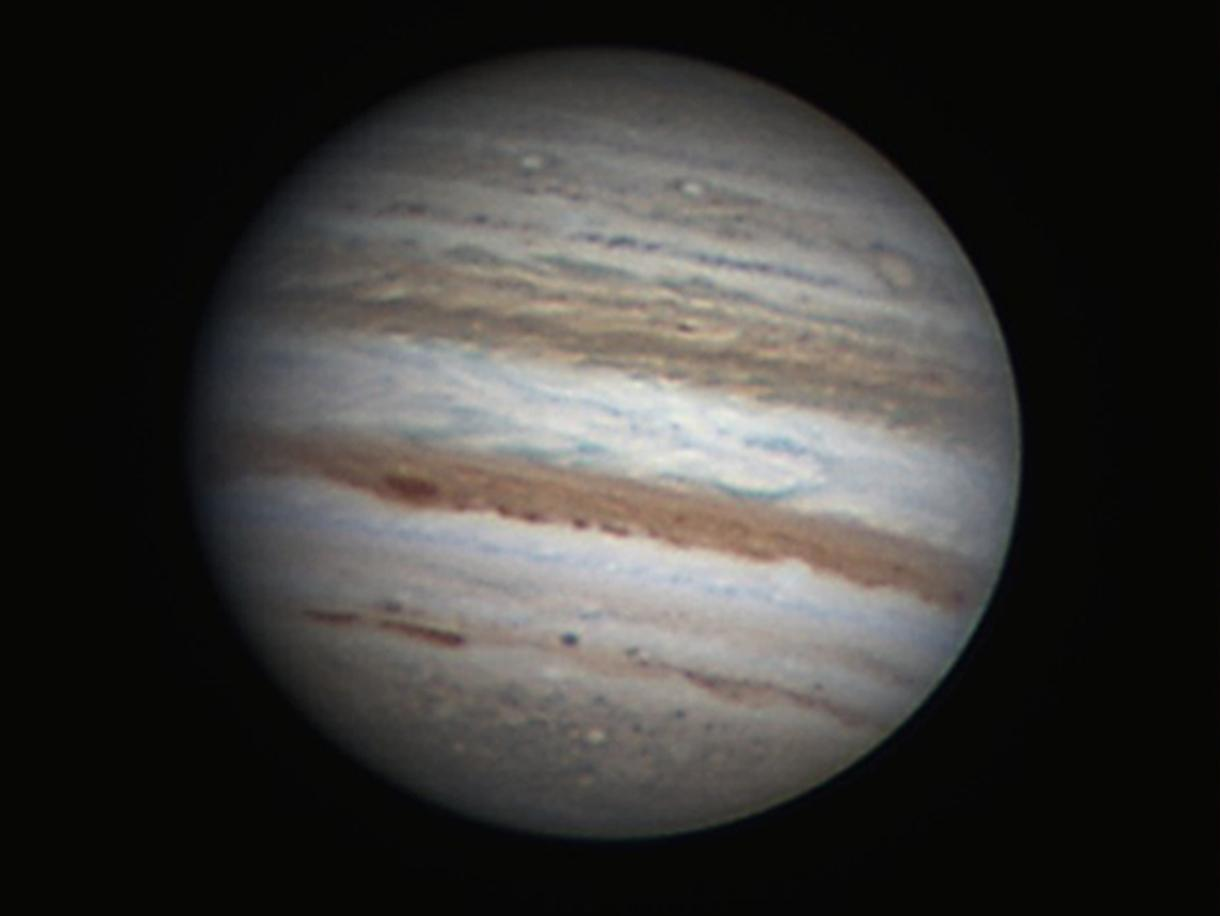
\includegraphics[width=0.7\textwidth]{img/realzado.jpg}
			\caption{Imagen inicial realzado}
			\label{img: realzado src}
		\end{center}
	\end{figure}

	\noindent Para realzar la imagen podemos aplicar filtros directamente sobre la imagen original. En este caso, hemos aplicado un preajuste del histograma, para hacer que el margen dinámico ocupe todo el histograma. Una vez tenemos la imagen preajustada, la filtramos con \texttt{prewitt} o \texttt{sobel}.
	
	\begin{lstlisting}[language=Matlab, caption={Implementación de filtros para el realzado en MATLAB}]
% 5 - Realzado
% Enrique
clear;

img_rgb = imread('realzado.jpg');

% Preajuste expansion margen dinamico
img_adj = imadjust(img_rgb, stretchlim(img_rgb), [ ]);

% Caso uno, prewitt
filter = fspecial('prewitt');
img_filtered = imfilter(img_adj, filter, 'replicate');
%img_rgb_1 = imadd(img_adj, img_filtered);
img_rgb_1 = img_adj - img_filtered;

% Caso dos, sobel
filter = fspecial('sobel');
img_filtered = imfilter(img_adj, filter, 'replicate');
%img_rgb_2 = imadd(img_adj, img_filtered);
img_rgb_2 = img_adj - img_filtered;

figure
subplot(2,2,1)
imshow(img_rgb, [])
title('Imagen original')

subplot(2,2,2)
imshow(img_adj, [])
title('Imagen preadjustada')

subplot(2,2,3)
imshow(img_rgb_1, [])
title('Imagen realzada (prewitt)')

subplot(2,2,4)
imshow(img_rgb_2, [])
title('Imagen realzada (sobel)')

	\end{lstlisting}

	%\vspace{10px};
	\pagebreak
	
	\noindent Una vez ejecutado el código, obtenemos como salida una figura comparativa entre la imagen original, la imagen preajustada y las opciones de filtrado (\texttt{prewitt} y \texttt{sobel}).
	
	\begin{figure}[h]
		\begin{center}
			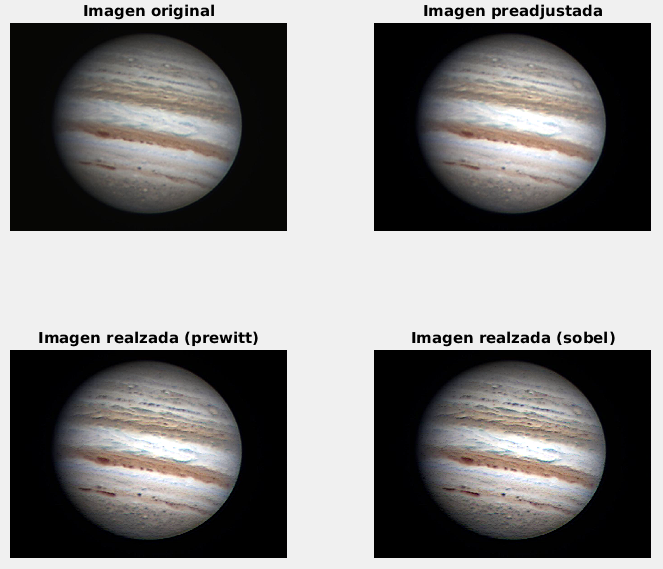
\includegraphics[width=0.9\textwidth]{img/realzado_output.png}
			\caption{Imagen inicial ruido}
			\label{img: realzado output}
		\end{center}
	\end{figure}

	\noindent Si tuvieramos que quedarnos con uno de los filtrados, el filtro \texttt{sobel} parece que realza mucho más las transiciones de color, cosa que en el caso de \texttt{prewitt} también distinguimos, pero en esta imagen en concreto el realzado es menor que respecto a \texttt{sobel}.
	
	\pagebreak
	
	\section{Ruido}
	
	\noindent En este ejercicio tenemos que aplicar técnicas de reducción de ruido a la imagen \ref{img: ruido src}. Lo primero que tendríamos que intentar hacer es ver que tipo de ruido es, en este caso creemos que es ruido tipo ``sal y pimienta''.
	
	\begin{figure}[h]
		\begin{center}
			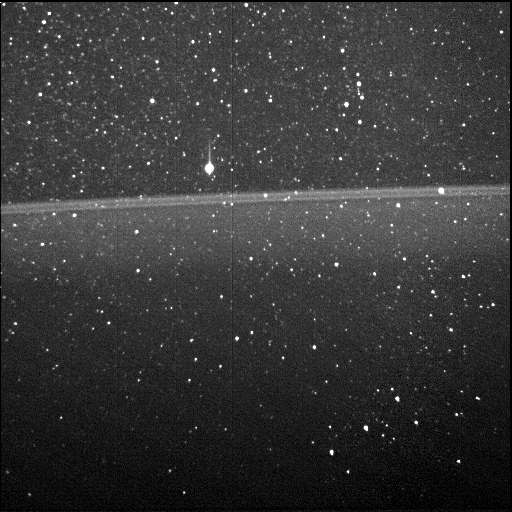
\includegraphics[width=0.7\textwidth]{img/ruido.jpg}
			\caption{Imagen inicial ruido}
			\label{img: ruido src}
		\end{center}
	\end{figure}
	
	\noindent Puesto que el ruido de la imagen se puede entender como un ruido de tipo ``sal y pimienta'', una de las técnicas que podemos utilizar es ejecutar de manera recursiva un filtro de mediana sobre la imagen.
	
	\begin{lstlisting}[language=Matlab, caption={Implementación filtro mediana para reducir ruido en MATLAB}]
% 6 - Ruido Sal y Pimienta
% Enrique
clear;

img_rgb = 'ruido.jpg';
neighborn = 4;
times = 5;

img = imread(img_rgb);
img = mat2gray(img,[0 255]);
img = rgb2gray(img);

figure
subplot(1,2,1)
imshow(img, [])
title('Imagen original [RGB]')

% Aplicamos filtro mediana
img_median = img;
for n=1:times,
img_median = medfilt2(img_median, [1 1]*neighborn);
end

% Representamos resultado
subplot(1,2,2)
imshow(img_median, []),
axis off image,
title(['Imagen eliminado el ruido usando filtro mediana con N=' num2str(neighborn) ' T=' num2str(times) ])
	\end{lstlisting}

	\vspace{10px}

	\noindent Una vez ejecutado el código, tendremos como salida una comparativa entre la imagen inicial (ver figura \ref{img: ruido src}) y imagen resultante tras eliminar el ruido ``sal y pimienta'':
	
	\begin{figure}[h]
		\begin{center}
			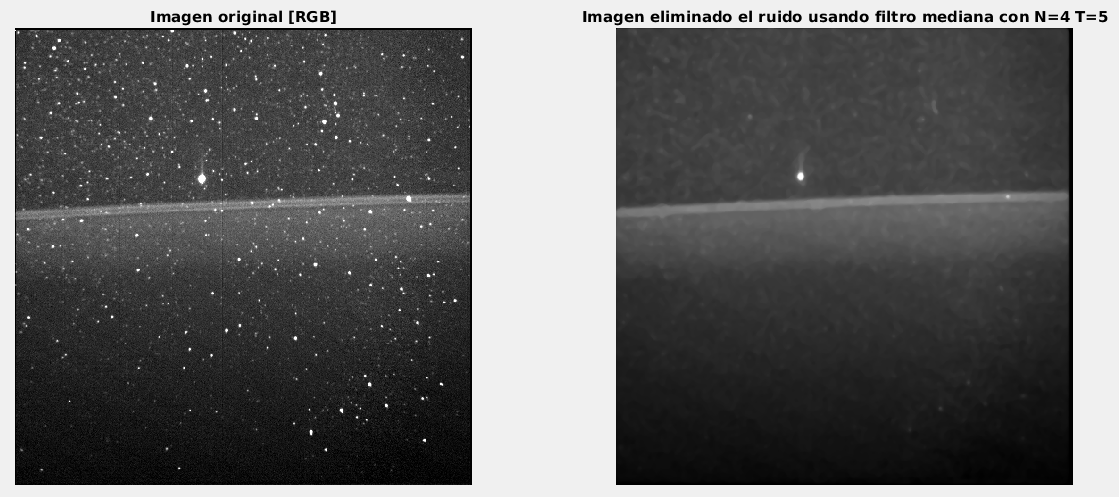
\includegraphics[width=1\textwidth]{img/ruido_output.png}
			\caption{Figura de salida al ejecutar script de MATLAB \texttt{ruido.m}}
			\label{img: ruido output}
		\end{center}
	\end{figure}
	
	\pagebreak
	
	\section{Patrones}
	
	\pagebreak
	
	\section{Pseudocoloración}
	
	\noindent En este ejercicio tenemos que aplicar técnicas de pseudocoloración a la imagen de un planeta (ver Figura X), con esto pretendemos ver detalles, que en el caso de ver la imagen en niveles de gris no veríamos.
	
	\begin{figure}[h]
		\begin{center}
			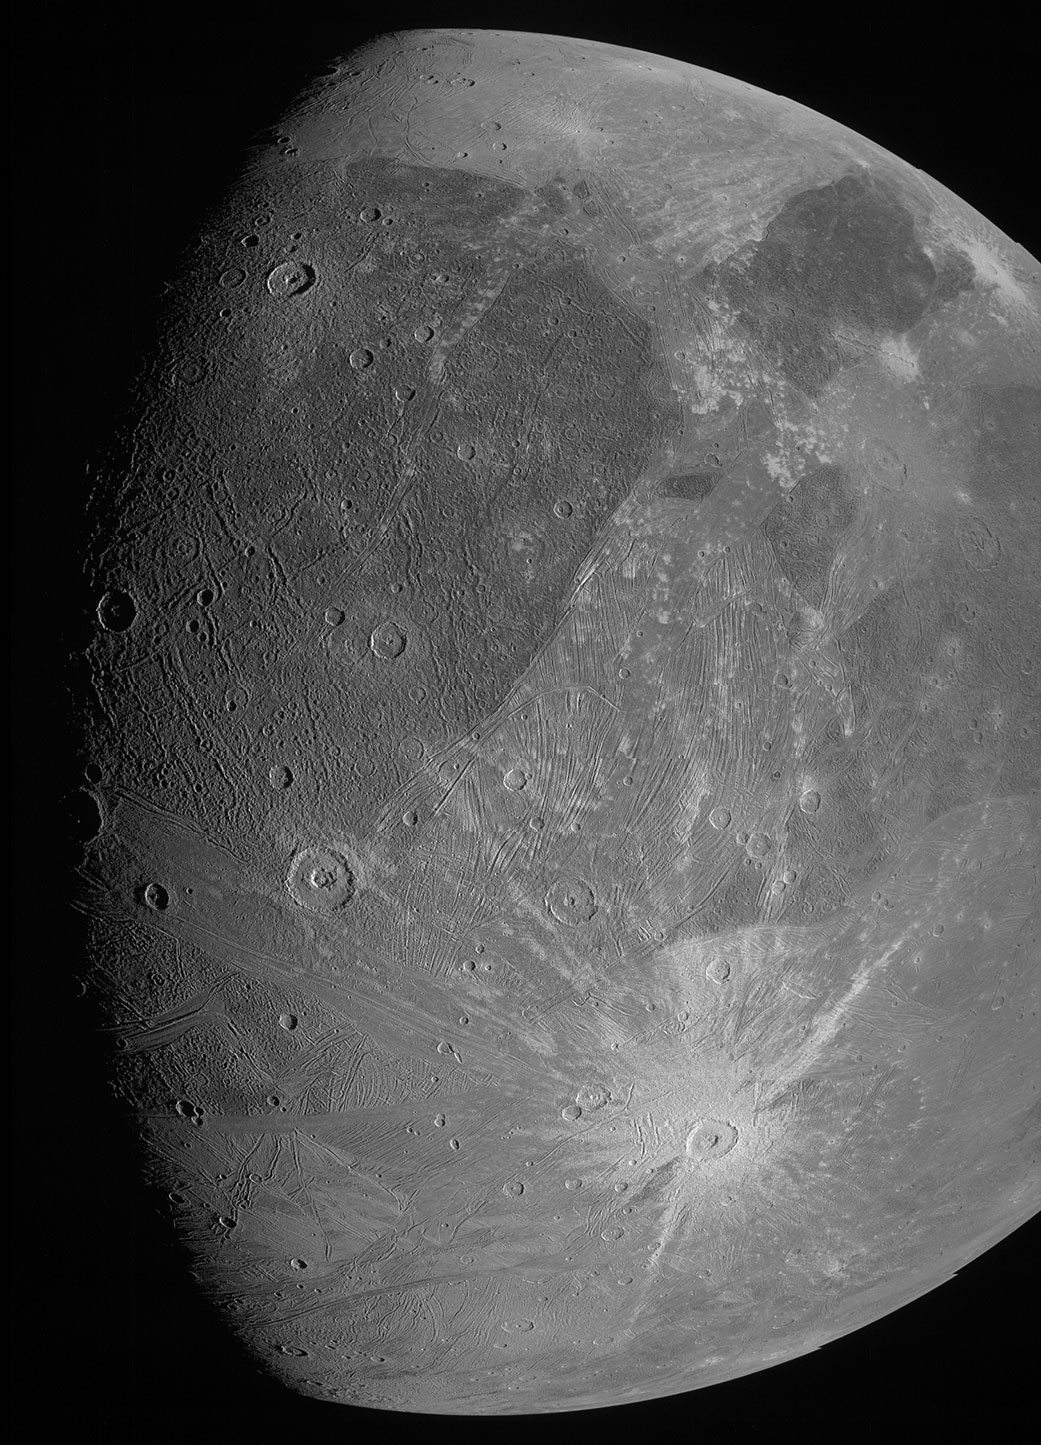
\includegraphics[width=0.4\textwidth]{img/pseudocoloracion.jpg}
			\caption{Imagen inicial pseudocoloración}
			\label{img: pseudocoloración src}
		\end{center}
	\end{figure}

	\noindent Para la resolución de este ejercicio hemos usado la técnica de coloración de una imagen dependiendo de su nivel de gris. Para ello, hemos probado todos los mapas de colores que MATLAB nos ofrece, sin embargo solo \texttt{copper}, \texttt{pink}, \texttt{bone}, \texttt{hot} y \texttt{parula} nos aportaban resultados útiles.
	
	\begin{lstlisting}[language=Matlab, caption={Implementación de pseucoloración en MATLAB}]
		% 8 - Pseudocoloracion por nivel de gris
		% Enrique 
		
		img_rgb = 'pseudocoloracion.jpg';
		gray_lvl = 64;
		
		img = imread(img_rgb);
		img = mat2gray(img,[0 255]);
		img = rgb2gray(img);
		
		% Utilizamos 64 niveles de gris
		img_colored = grayslice(img, gray_lvl);
		
		
		% Representamos cada una de las coloraciones
		figure
		subplot(2,3,1),
		subimage(img);
		axis off image,
		title('Imagen original en escala de gris')
		
		subplot(2,3,2),
		subimage(img_colored, copper(gray_lvl));
		axis off image,
		title('Pseudocoloracion (copper)')
		
		subplot(2,3,3),
		subimage(img_colored, pink(gray_lvl));
		axis off image,
		title('Pseudocoloracion (pink)')
		
		subplot(2,3,4),
		subimage(img_colored, bone(gray_lvl));
		axis off image,
		title('Pseudocoloracion (bone)')
		
		subplot(2,3,5),
		subimage(img_colored, hot(gray_lvl));
		axis off image,
		title('Pseudocoloracion (hot)')
		
		subplot(2,3,6),
		subimage(img_colored, parula(gray_lvl));
		axis off image,
		title('Pseudocoloracion (parula)')
	\end{lstlisting}
	
	%\vspace{10px}
	\pagebreak
	
	\noindent Una vez ejecutado el código, tendremos como salida una comparativa entre la imagen inicial (ver figura \ref{img: pseudocoloración src}) y las diferentes imágenes resultantes tras aplicar pseudocoloración:
	
	\begin{figure}[h]
		\begin{center}
			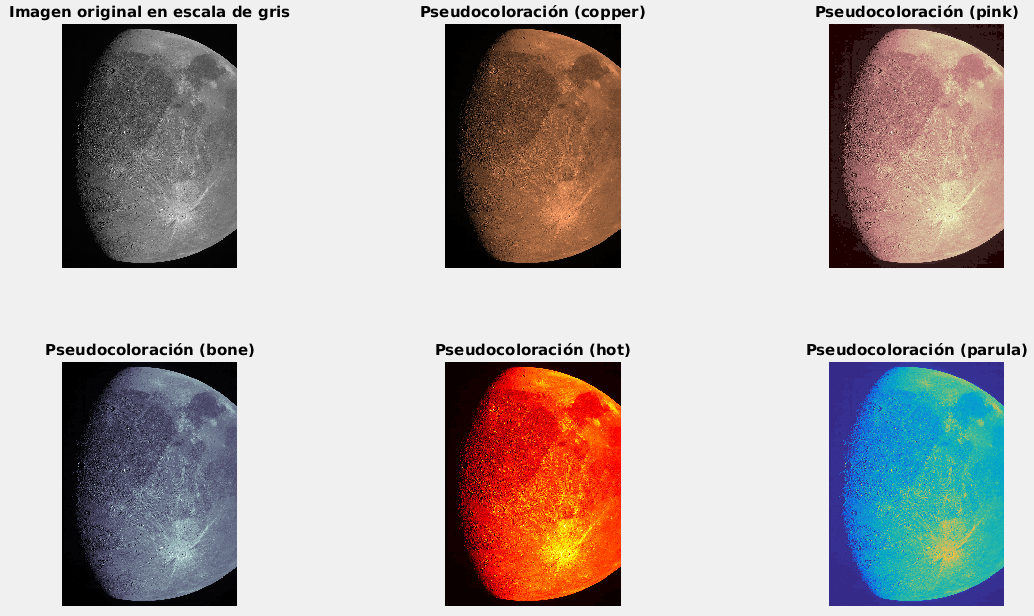
\includegraphics[width=1\textwidth]{img/pseudocoloracion_output.png}
			\caption{Figura de salida al ejecutar script de MATLAB \texttt{pseudocoloracion.m}}
			\label{img: pseudocoloracion output}
		\end{center}
	\end{figure}

	\noindent Si tuviera que elegir entre alguna de las imágenes obtenidas, considero que con \texttt{hot} y \texttt{parula} podemos distinguir más detalles, sin embargo el resto de coloraciones también aportan más detalle que la original.
	
	\pagebreak
\end{document}